% A LaTeX template for MSc Thesis submissions to 
% Politecnico di Milano (PoliMi) - School of Industrial and Information Engineering
%
% S. Bonetti, A. Gruttadauria, G. Mescolini, A. Zingaro
% e-mail: template-tesi-ingind@polimi.it
%
% Last Revision: October 2021
%
% Copyright 2021 Politecnico di Milano, Italy. NC-BY

\documentclass{Configuration_Files/PoliMi3i_thesis}

%------------------------------------------------------------------------------
%	REQUIRED PACKAGES AND  CONFIGURATIONS
%------------------------------------------------------------------------------

% CONFIGURATIONS
\usepackage{parskip} % For paragraph layout
\usepackage{setspace} % For using single or double spacing
\usepackage{emptypage} % To insert empty pages
\usepackage{multicol} % To write in multiple columns (executive summary)
\setlength\columnsep{15pt} % Column separation in executive summary
\setlength\parindent{0pt} % Indentation
\raggedbottom  

% PACKAGES FOR TITLES
\usepackage{titlesec}
% \titlespacing{\section}{left spacing}{before spacing}{after spacing}
\titlespacing{\section}{0pt}{3.3ex}{2ex}
\titlespacing{\subsection}{0pt}{3.3ex}{1.65ex}
\titlespacing{\subsubsection}{0pt}{3.3ex}{1ex}
\usepackage{color}

% PACKAGES FOR LANGUAGE AND FONT
\usepackage[english]{babel} % The document is in English  
\usepackage[utf8]{inputenc} % UTF8 encoding
\usepackage[T1]{fontenc} % Font encoding
\usepackage[11pt]{moresize} % Big fonts

% PACKAGES FOR IMAGES
\usepackage{graphicx}
\usepackage{transparent} % Enables transparent images
\usepackage{eso-pic} % For the background picture on the title page
\usepackage{subfig} % Numbered and caption subfigures using \subfloat.
\usepackage{tikz} % A package for high-quality hand-made figures.
\usetikzlibrary{}
\graphicspath{{./Images/}} % Directory of the images
\usepackage{caption} % Coloured captions
\usepackage{xcolor} % Coloured captions
\usepackage{amsthm,thmtools,xcolor} % Coloured "Theorem"
\usepackage{float}

% STANDARD MATH PACKAGES
\usepackage{amsmath}
\usepackage{amsthm}
\usepackage{amssymb}
\usepackage{amsfonts}
\usepackage{bm}
\usepackage[overload]{empheq} % For braced-style systems of equations.
\usepackage{fix-cm} % To override original LaTeX restrictions on sizes

% PACKAGES FOR TABLES
\usepackage{tabularx}
\usepackage{longtable} % Tables that can span several pages
\usepackage{colortbl}

% PACKAGES FOR ALGORITHMS (PSEUDO-CODE)
\usepackage{algorithm}
\usepackage{algorithmic}

% PACKAGES FOR REFERENCES & BIBLIOGRAPHY
\usepackage[colorlinks=true,linkcolor=black,anchorcolor=black,citecolor=black,filecolor=black,menucolor=black,runcolor=black,urlcolor=black]{hyperref} % Adds clickable links at references
\usepackage{cleveref}
\usepackage[square, numbers, sort&compress]{natbib} % Square brackets, citing references with numbers, citations sorted by appearance in the text and compressed
\bibliographystyle{abbrvnat} % You may use a different style adapted to your field

% OTHER PACKAGES
\usepackage{pdfpages} % To include a pdf file
\usepackage{afterpage}
\usepackage{lipsum} % DUMMY PACKAGE
\usepackage{fancyhdr} % For the headers
\fancyhf{}

% Input of configuration file. Do not change config.tex file unless you really know what you are doing. 
% Define blue color typical of polimi
\definecolor{bluepoli}{cmyk}{0.4,0.1,0,0.4}

% Custom theorem environments
\declaretheoremstyle[
  headfont=\color{bluepoli}\normalfont\bfseries,
  bodyfont=\color{black}\normalfont\itshape,
]{colored}

% Set-up caption colors
\captionsetup[figure]{labelfont={color=bluepoli}} % Set colour of the captions
\captionsetup[table]{labelfont={color=bluepoli}} % Set colour of the captions
\captionsetup[algorithm]{labelfont={color=bluepoli}} % Set colour of the captions

\theoremstyle{colored}
\newtheorem{theorem}{Theorem}[chapter]
\newtheorem{proposition}{Proposition}[chapter]

% Enhances the features of the standard "table" and "tabular" environments.
\newcommand\T{\rule{0pt}{2.6ex}}
\newcommand\B{\rule[-1.2ex]{0pt}{0pt}}

% Pseudo-code algorithm descriptions.
\newcounter{algsubstate}
\renewcommand{\thealgsubstate}{\alph{algsubstate}}
\newenvironment{algsubstates}
  {\setcounter{algsubstate}{0}%
   \renewcommand{\STATE}{%
     \stepcounter{algsubstate}%
     \Statex {\small\thealgsubstate:}\space}}
  {}

% New font size
\newcommand\numfontsize{\@setfontsize\Huge{200}{60}}

% Title format: chapter
\titleformat{\chapter}[hang]{
\fontsize{50}{20}\selectfont\bfseries\filright}{\textcolor{bluepoli} \thechapter\hsp\hspace{2mm}\textcolor{bluepoli}{|   }\hsp}{0pt}{\huge\bfseries \textcolor{bluepoli}
}

% Title format: section
\titleformat{\section}
{\color{bluepoli}\normalfont\Large\bfseries}
{\color{bluepoli}\thesection.}{1em}{}

% Title format: subsection
\titleformat{\subsection}
{\color{bluepoli}\normalfont\large\bfseries}
{\color{bluepoli}\thesubsection.}{1em}{}

% Title format: subsubsection
\titleformat{\subsubsection}
{\color{bluepoli}\normalfont\large\bfseries}
{\color{bluepoli}\thesubsubsection.}{1em}{}

% Shortening for setting no horizontal-spacing
\newcommand{\hsp}{\hspace{0pt}}

\makeatletter
% Renewcommand: cleardoublepage including the background pic
\renewcommand*\cleardoublepage{%
  \clearpage\if@twoside\ifodd\c@page\else
  \null
  \AddToShipoutPicture*{\BackgroundPic}
  \thispagestyle{empty}%
  \newpage
  \if@twocolumn\hbox{}\newpage\fi\fi\fi}
\makeatother

%For correctly numbering algorithms
\numberwithin{algorithm}{chapter}

%----------------------------------------------------------------------------
%	NEW COMMANDS DEFINED
%----------------------------------------------------------------------------

% EXAMPLES OF NEW COMMANDS
\newcommand{\bea}{\begin{eqnarray}} % Shortcut for equation arrays
\newcommand{\eea}{\end{eqnarray}}
\newcommand{\e}[1]{\times 10^{#1}}  % Powers of 10 notation

%----------------------------------------------------------------------------
%	ADD YOUR PACKAGES (be careful of package interaction)
%----------------------------------------------------------------------------

%----------------------------------------------------------------------------
%	ADD YOUR DEFINITIONS AND COMMANDS (be careful of existing commands)
%----------------------------------------------------------------------------

%----------------------------------------------------------------------------
%	BEGIN OF YOUR DOCUMENT
%----------------------------------------------------------------------------

\begin{document}

\fancypagestyle{plain}{%
\fancyhf{} % Clear all header and footer fields
\fancyhead[RO,RE]{\thepage} %RO=right odd, RE=right even
\renewcommand{\headrulewidth}{0pt}
\renewcommand{\footrulewidth}{0pt}}

%----------------------------------------------------------------------------
%	TITLE PAGE
%----------------------------------------------------------------------------

\pagestyle{empty} % No page numbers
\frontmatter % Use roman page numbering style (i, ii, iii, iv...) for the preamble pages

\puttitle{
	title=Systems and Methods for Big and Unstructured Data Project,
	name1=Gabriele Ginestroni, % Author Name and Surname
	name2=Giacomo Gumiero,
	name3=Lorenzo Iovine,
	name4=Nicola Landini,
	name5=Francesco Leone,
	academicyear=2022-2023,
	groupnumber=10
} % These info will be put into your Title page 

%----------------------------------------------------------------------------
%	PREAMBLE PAGES: ABSTRACT (inglese e italiano), EXECUTIVE SUMMARY
%----------------------------------------------------------------------------
\startpreamble
\setcounter{page}{1} % Set page counter to 1

%----------------------------------------------------------------------------
%	LIST OF CONTENTS/FIGURES/TABLES/SYMBOLS
%----------------------------------------------------------------------------

% TABLE OF CONTENTS
\thispagestyle{empty}
\tableofcontents % Table of contents 
\thispagestyle{empty}
\cleardoublepage

%-------------------------------------------------------------------------
%	THESIS MAIN TEXT
%-------------------------------------------------------------------------
% In the main text of your thesis you can write the chapters in two different ways:
%
%(1) As presented in this template you can write:
%    \chapter{Title of the chapter}
%    *body of the chapter*
%
%(2) You can write your chapter in a separated .tex file and then include it in the main file with the following command:
%    \chapter{Title of the chapter}
%    \input{chapter_file.tex}
%
% Especially for long thesis, we recommend you the second option.

\addtocontents{toc}{\vspace{2em}} % Add a gap in the Contents, for aesthetics
\mainmatter % Begin numeric (1,2,3...) page numbering

\chapter{Introduction}
\label{ch:introduction}%
% The \label{...}% enables to remove the small indentation that is generated, always leave the % symbol.

In this chapter will be presented the problem specification and the hypothesis under which the database is implemented.

\section{Problem Specification}
\label{sec:prob_specs}
This project aims to build an Information System that handles scientific articles contained in the DBLP
bibliography. The project involves managing the type of the articles and the associated DOI (Digital Object Identifier),
which identifies an article or a document and links to it on the web. Other entities to deal with are authors, identified by
an ID or ORCID (Open Researcher and Contributor ID), and their affiliations with organizations. In order to address the
problem, we will store data in a graph database, allowing us to visualize relations and handle information correctly.


\section{Assumptions}
\label{sec:assumptions}
\begin{enumerate}
    \item All the data in the dataset are heterogeneous, so fields are different
    \item The \textbf{authors} with missing field \emph{\_id} are not considered
    \item It is possible that an author writes for different organizations
    \item Field \emph{\_id} in \textbf{author} is unique
    \item Field \emph{\_id} in \textbf{article} exists and it is unique
    \item It is impossible that 2 different articles are on the same journal, in the same \emph{volume} with an intersection between \emph{page\_start} and \emph{page\_end}
    \item The designed model doesn't take into consideration the URL associated to the article node, as the main focus of the project was not reading the article
    \item It is possible to find a self-reference in a publication
    \item A \emph{venue} can be instantiated as a journal, a conference or a generic venue!!!!!!!!
\end{enumerate}

\chapter{ER Diagram}
\begin{figure}[H]
    \centering
    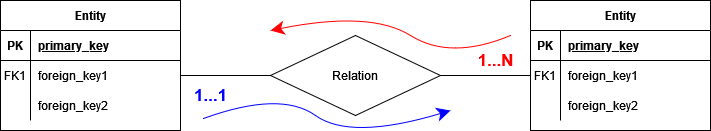
\includegraphics[width=0.6\textwidth]{legendaER.png}
    \caption{ER Diagram Organization}
    \label{fig:erleg}
\end{figure}
\bigskip
\begin{figure}[H]
    \centering
    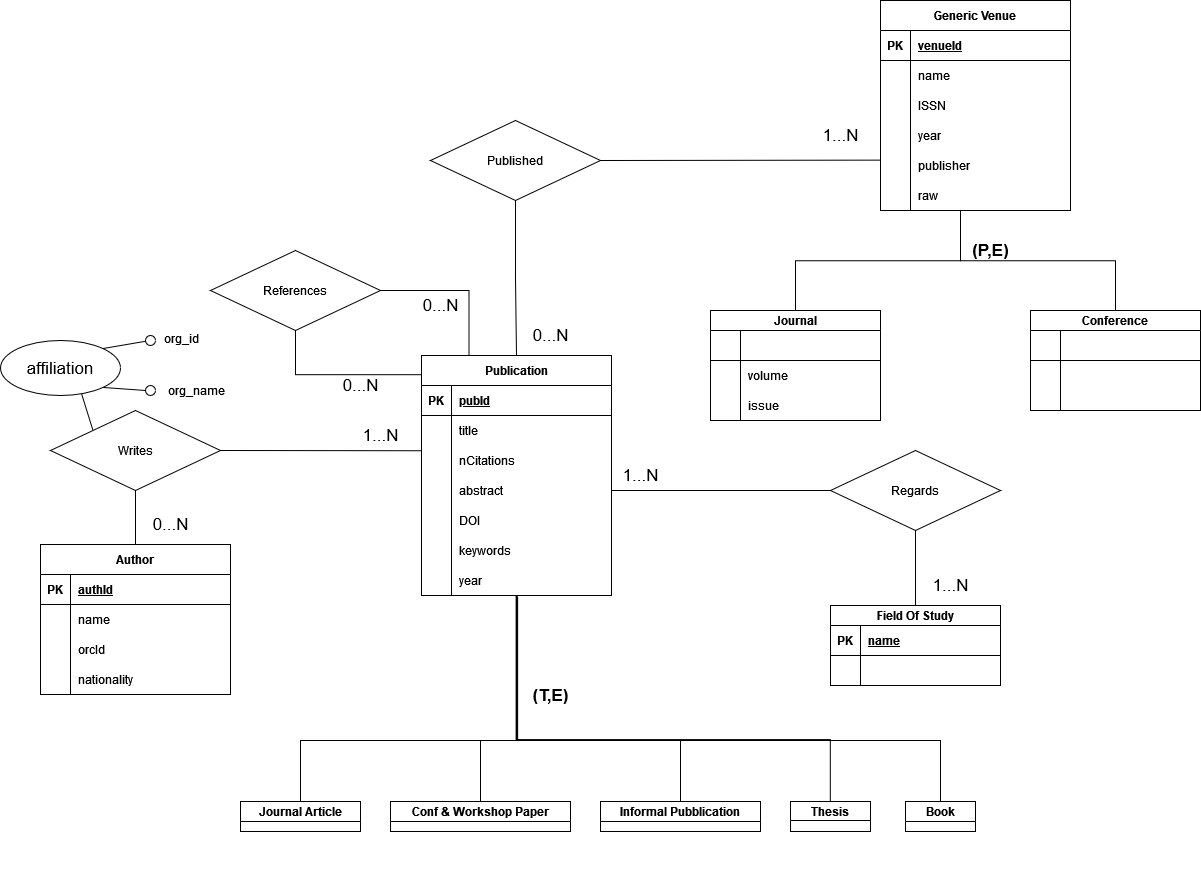
\includegraphics[width=1\textwidth]{ER.png}
    \caption{ER Diagram}
    \label{fig:er}
\end{figure}

\newpage
The ER diagram designed contains the following entities:
\begin{itemize}
    \item \textbf{Publication:} this entity represents all the scientific articles. They are identified by their primary key \emph{\_id}
            and other important attributes are: \emph{DOI, title, last\_edit\_data, abstract, keywords, pages, pub\_date}.
            Of course the attributes of such entity could be enlarged, but as a sample dataset we have believed these are enough.
            Publication entity is the superclass of a Total and Exclusive ISA relationship with the following subclasses:
            \emph{Journal article, Conference \& Workshop paper, Informal publication, Thesis, Book}
    \item \textbf{Author:} it represents all the people that submitted at least one publication. Its primary key is \emph{\_id} and the
            foreign keys are: \emph{name, surname, nationality, paperCount, citationCount}.
            Of course the attributes of such entity could be enlarged, but as a sample dataset we have believed these are enough
    \item \textbf{Venue:} it's the entity that represents the type of a publication. This is a superclass that creates a Partial and Exclusive
            ISA relationship with the two subclasses \emph{Journal} and \emph{Conference}.
            The primary key is \emph{raw} and the other keys are: \emph{name, date, venue\_id}
    \item \textbf{Field Of Study:} this entity represents the topics of the related publication
\end{itemize}
\bigskip

The ER diagram designed contains the following relationships:
\begin{itemize}
    \item \textbf{Writes:} is the relationship between \emph{author} and \emph{publication} which specifies also the affiliation
            with the org\_id and the org\_name
    \item \textbf{Mentions:} occurs between two \emph{publication} and specifies when a publication refers to another one
    \item \textbf{Is about:} binds a \emph{publication} with its \emph{fields of study}
    \item \textbf{Published on:} simply relates a \emph{publication} to its \emph{venue}
\end{itemize}

\chapter{Dataset Description}

\chapter{Graph Diagram}

\chapter{Queries and Commands}

\chapter{Conclusion}

%-------------------------------------------------------------------------
%	APPENDICES
%-------------------------------------------------------------------------

\cleardoublepage
\addtocontents{toc}{\vspace{2em}} % Add a gap in the Contents, for aesthetics
\appendix
\chapter{Appendix A}
If you need to include an appendix to support the research in your thesis, you can place it at the end of the manuscript.
An appendix contains supplementary material (figures, tables, data, codes, mathematical proofs, surveys, \dots)
which supplement the main results contained in the previous chapters.


% LIST OF FIGURES
\listoffigures

% LIST OF TABLES
\listoftables

\cleardoublepage

\end{document}
